% Created by tikzDevice version 0.12.3.1 on 2022-05-02 11:32:15
% !TEX encoding = UTF-8 Unicode
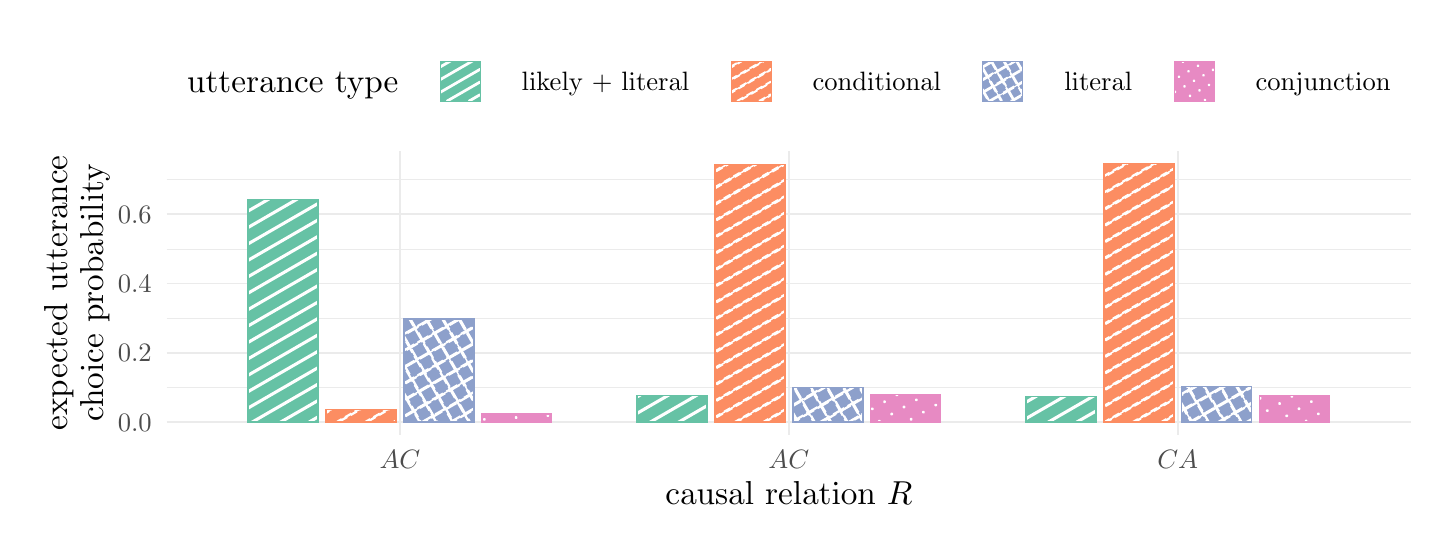
\begin{tikzpicture}[x=1pt,y=1pt]
\definecolor{fillColor}{RGB}{255,255,255}
\path[use as bounding box,fill=fillColor,fill opacity=0.00] (0,0) rectangle (505.89,180.67);
\begin{scope}
\path[clip] ( 50.22, 33.48) rectangle (499.89,136.22);
\definecolor{drawColor}{gray}{0.92}

\path[draw=drawColor,line width= 0.3pt,line join=round] ( 50.22, 50.66) --
	(499.89, 50.66);

\path[draw=drawColor,line width= 0.3pt,line join=round] ( 50.22, 75.69) --
	(499.89, 75.69);

\path[draw=drawColor,line width= 0.3pt,line join=round] ( 50.22,100.72) --
	(499.89,100.72);

\path[draw=drawColor,line width= 0.3pt,line join=round] ( 50.22,125.75) --
	(499.89,125.75);

\path[draw=drawColor,line width= 0.6pt,line join=round] ( 50.22, 38.15) --
	(499.89, 38.15);

\path[draw=drawColor,line width= 0.6pt,line join=round] ( 50.22, 63.18) --
	(499.89, 63.18);

\path[draw=drawColor,line width= 0.6pt,line join=round] ( 50.22, 88.21) --
	(499.89, 88.21);

\path[draw=drawColor,line width= 0.6pt,line join=round] ( 50.22,113.24) --
	(499.89,113.24);

\path[draw=drawColor,line width= 0.6pt,line join=round] (134.53, 33.48) --
	(134.53,136.22);

\path[draw=drawColor,line width= 0.6pt,line join=round] (275.06, 33.48) --
	(275.06,136.22);

\path[draw=drawColor,line width= 0.6pt,line join=round] (415.58, 33.48) --
	(415.58,136.22);
\definecolor{fillColor}{RGB}{102,194,165}

\path[fill=fillColor] ( 79.73, 38.15) rectangle (105.02,118.55);
\definecolor{fillColor}{RGB}{252,141,98}

\path[fill=fillColor] (107.83, 38.15) rectangle (133.13, 42.70);
\definecolor{fillColor}{RGB}{141,160,203}

\path[fill=fillColor] (135.94, 38.15) rectangle (161.23, 75.47);
\definecolor{fillColor}{RGB}{231,138,195}

\path[fill=fillColor] (164.04, 38.15) rectangle (189.34, 41.03);
\definecolor{fillColor}{RGB}{102,194,165}

\path[fill=fillColor] (220.25, 38.15) rectangle (245.55, 47.77);
\definecolor{fillColor}{RGB}{252,141,98}

\path[fill=fillColor] (248.36, 38.15) rectangle (273.65,131.20);
\definecolor{fillColor}{RGB}{141,160,203}

\path[fill=fillColor] (276.46, 38.15) rectangle (301.75, 50.61);
\definecolor{fillColor}{RGB}{231,138,195}

\path[fill=fillColor] (304.57, 38.15) rectangle (329.86, 48.16);
\definecolor{fillColor}{RGB}{102,194,165}

\path[fill=fillColor] (360.77, 38.15) rectangle (386.07, 47.42);
\definecolor{fillColor}{RGB}{252,141,98}

\path[fill=fillColor] (388.88, 38.15) rectangle (414.17,131.55);
\definecolor{fillColor}{RGB}{141,160,203}

\path[fill=fillColor] (416.98, 38.15) rectangle (442.28, 50.98);
\definecolor{fillColor}{RGB}{231,138,195}

\path[fill=fillColor] (445.09, 38.15) rectangle (470.38, 47.78);
\definecolor{drawColor}{RGB}{255,255,255}
\definecolor{fillColor}{RGB}{255,255,255}

\path[draw=drawColor,line width= 0.6pt,line join=round,line cap=rect,fill=fillColor] (101.18, 38.15) --
	(105.02, 40.37) --
	(105.02, 39.77) --
	(102.21, 38.15) --
	(101.18, 38.15) --
	cycle;

\path[draw=drawColor,line width= 0.6pt,line join=round,line cap=rect,fill=fillColor] ( 90.90, 38.15) --
	(105.02, 46.30) --
	(105.02, 45.70) --
	( 91.93, 38.15) --
	( 90.90, 38.15) --
	cycle;

\path[draw=drawColor,line width= 0.6pt,line join=round,line cap=rect,fill=fillColor] ( 80.63, 38.15) --
	(105.02, 52.23) --
	(105.02, 51.64) --
	( 81.66, 38.15) --
	( 80.63, 38.15) --
	cycle;

\path[draw=drawColor,line width= 0.6pt,line join=round,line cap=rect,fill=fillColor] ( 79.73, 43.56) --
	(105.02, 58.16) --
	(105.02, 57.57) --
	( 79.73, 42.96) --
	( 79.73, 43.56) --
	cycle;

\path[draw=drawColor,line width= 0.6pt,line join=round,line cap=rect,fill=fillColor] ( 79.73, 49.49) --
	(105.02, 64.09) --
	(105.02, 63.50) --
	( 79.73, 48.90) --
	( 79.73, 49.49) --
	cycle;

\path[draw=drawColor,line width= 0.6pt,line join=round,line cap=rect,fill=fillColor] ( 79.73, 55.42) --
	(105.02, 70.03) --
	(105.02, 69.43) --
	( 79.73, 54.83) --
	( 79.73, 55.42) --
	cycle;

\path[draw=drawColor,line width= 0.6pt,line join=round,line cap=rect,fill=fillColor] ( 79.73, 61.35) --
	(105.02, 75.96) --
	(105.02, 75.36) --
	( 79.73, 60.76) --
	( 79.73, 61.35) --
	cycle;

\path[draw=drawColor,line width= 0.6pt,line join=round,line cap=rect,fill=fillColor] ( 79.73, 67.29) --
	(105.02, 81.89) --
	(105.02, 81.30) --
	( 79.73, 66.69) --
	( 79.73, 67.29) --
	cycle;

\path[draw=drawColor,line width= 0.6pt,line join=round,line cap=rect,fill=fillColor] ( 79.73, 73.22) --
	(105.02, 87.82) --
	(105.02, 87.23) --
	( 79.73, 72.63) --
	( 79.73, 73.22) --
	cycle;

\path[draw=drawColor,line width= 0.6pt,line join=round,line cap=rect,fill=fillColor] ( 79.73, 79.15) --
	(105.02, 93.75) --
	(105.02, 93.16) --
	( 79.73, 78.56) --
	( 79.73, 79.15) --
	cycle;

\path[draw=drawColor,line width= 0.6pt,line join=round,line cap=rect,fill=fillColor] ( 79.73, 85.08) --
	(105.02, 99.69) --
	(105.02, 99.09) --
	( 79.73, 84.49) --
	( 79.73, 85.08) --
	cycle;

\path[draw=drawColor,line width= 0.6pt,line join=round,line cap=rect,fill=fillColor] ( 79.73, 91.01) --
	(105.02,105.62) --
	(105.02,105.02) --
	( 79.73, 90.42) --
	( 79.73, 91.01) --
	cycle;

\path[draw=drawColor,line width= 0.6pt,line join=round,line cap=rect,fill=fillColor] ( 79.73, 96.95) --
	(105.02,111.55) --
	(105.02,110.96) --
	( 79.73, 96.35) --
	( 79.73, 96.95) --
	cycle;

\path[draw=drawColor,line width= 0.6pt,line join=round,line cap=rect,fill=fillColor] ( 79.73,102.88) --
	(105.02,117.48) --
	(105.02,116.89) --
	( 79.73,102.29) --
	( 79.73,102.88) --
	cycle;

\path[draw=drawColor,line width= 0.6pt,line join=round,line cap=rect,fill=fillColor] ( 79.73,108.81) --
	( 96.59,118.55) --
	( 97.62,118.55) --
	( 79.73,108.22) --
	( 79.73,108.81) --
	cycle;

\path[draw=drawColor,line width= 0.6pt,line join=round,line cap=rect,fill=fillColor] ( 79.73,114.74) --
	( 86.32,118.55) --
	( 87.35,118.55) --
	( 79.73,114.15) --
	( 79.73,114.74) --
	cycle;

\path[draw=drawColor,line width= 0.6pt,dash pattern=on 2pt off 2pt ,line join=round,line cap=rect,fill=fillColor] (132.00, 38.15) --
	(133.13, 38.80) --
	(133.13, 38.20) --
	(133.03, 38.15) --
	(132.00, 38.15) --
	cycle;

\path[draw=drawColor,line width= 0.6pt,dash pattern=on 2pt off 2pt ,line join=round,line cap=rect,fill=fillColor] (121.73, 38.15) --
	(129.61, 42.70) --
	(130.64, 42.70) --
	(122.76, 38.15) --
	(121.73, 38.15) --
	cycle;

\path[draw=drawColor,line width= 0.6pt,dash pattern=on 2pt off 2pt ,line join=round,line cap=rect,fill=fillColor] (111.45, 38.15) --
	(119.34, 42.70) --
	(120.36, 42.70) --
	(112.48, 38.15) --
	(111.45, 38.15) --
	cycle;

\path[draw=drawColor,line width= 0.6pt,dash pattern=on 2pt off 2pt ,line join=round,line cap=rect,fill=fillColor] (107.83, 41.99) --
	(109.06, 42.70) --
	(110.09, 42.70) --
	(107.83, 41.39) --
	(107.83, 41.99) --
	cycle;

\path[draw=drawColor,line width= 0.6pt,dash pattern=on 4pt off 2pt ,line join=round,line cap=rect,fill=fillColor] (152.55, 38.15) --
	(161.23, 43.16) --
	(161.23, 42.56) --
	(153.58, 38.15) --
	(152.55, 38.15) --
	cycle;

\path[draw=drawColor,line width= 0.6pt,dash pattern=on 4pt off 2pt ,line join=round,line cap=rect,fill=fillColor] (142.28, 38.15) --
	(161.23, 49.09) --
	(161.23, 48.50) --
	(143.31, 38.15) --
	(142.28, 38.15) --
	cycle;

\path[draw=drawColor,line width= 0.6pt,dash pattern=on 4pt off 2pt ,line join=round,line cap=rect,fill=fillColor] (135.94, 40.42) --
	(161.23, 55.02) --
	(161.23, 54.43) --
	(135.94, 39.82) --
	(135.94, 40.42) --
	cycle;

\path[draw=drawColor,line width= 0.6pt,dash pattern=on 4pt off 2pt ,line join=round,line cap=rect,fill=fillColor] (135.94, 46.35) --
	(161.23, 60.95) --
	(161.23, 60.36) --
	(135.94, 45.76) --
	(135.94, 46.35) --
	cycle;

\path[draw=drawColor,line width= 0.6pt,dash pattern=on 4pt off 2pt ,line join=round,line cap=rect,fill=fillColor] (135.94, 52.28) --
	(161.23, 66.89) --
	(161.23, 66.29) --
	(135.94, 51.69) --
	(135.94, 52.28) --
	cycle;

\path[draw=drawColor,line width= 0.6pt,dash pattern=on 4pt off 2pt ,line join=round,line cap=rect,fill=fillColor] (135.94, 58.21) --
	(161.23, 72.82) --
	(161.23, 72.22) --
	(135.94, 57.62) --
	(135.94, 58.21) --
	cycle;

\path[draw=drawColor,line width= 0.6pt,dash pattern=on 4pt off 2pt ,line join=round,line cap=rect,fill=fillColor] (135.94, 64.15) --
	(155.54, 75.47) --
	(156.57, 75.47) --
	(135.94, 63.55) --
	(135.94, 64.15) --
	cycle;

\path[draw=drawColor,line width= 0.6pt,dash pattern=on 4pt off 2pt ,line join=round,line cap=rect,fill=fillColor] (135.94, 70.08) --
	(145.27, 75.47) --
	(146.30, 75.47) --
	(135.94, 69.48) --
	(135.94, 70.08) --
	cycle;

\path[draw=drawColor,line width= 0.6pt,dash pattern=on 4pt off 2pt ,line join=round,line cap=rect,fill=fillColor] (136.02, 75.47) --
	(135.94, 75.42) --
	(135.94, 75.47) --
	(136.02, 75.47) --
	cycle;

\path[draw=drawColor,line width= 0.6pt,dash pattern=on 4pt off 2pt ,line join=round,line cap=rect,fill=fillColor] (135.94, 38.63) --
	(136.22, 38.15) --
	(135.94, 38.15) --
	(135.94, 38.63) --
	cycle;

\path[draw=drawColor,line width= 0.6pt,dash pattern=on 4pt off 2pt ,line join=round,line cap=rect,fill=fillColor] (135.94, 48.91) --
	(142.15, 38.15) --
	(141.56, 38.15) --
	(135.94, 47.88) --
	(135.94, 48.91) --
	cycle;

\path[draw=drawColor,line width= 0.6pt,dash pattern=on 4pt off 2pt ,line join=round,line cap=rect,fill=fillColor] (135.94, 59.18) --
	(148.08, 38.15) --
	(147.49, 38.15) --
	(135.94, 58.15) --
	(135.94, 59.18) --
	cycle;

\path[draw=drawColor,line width= 0.6pt,dash pattern=on 4pt off 2pt ,line join=round,line cap=rect,fill=fillColor] (135.94, 69.45) --
	(154.02, 38.15) --
	(153.42, 38.15) --
	(135.94, 68.43) --
	(135.94, 69.45) --
	cycle;

\path[draw=drawColor,line width= 0.6pt,dash pattern=on 4pt off 2pt ,line join=round,line cap=rect,fill=fillColor] (138.40, 75.47) --
	(159.95, 38.15) --
	(159.35, 38.15) --
	(137.81, 75.47) --
	(138.40, 75.47) --
	cycle;

\path[draw=drawColor,line width= 0.6pt,dash pattern=on 4pt off 2pt ,line join=round,line cap=rect,fill=fillColor] (144.33, 75.47) --
	(161.23, 46.19) --
	(161.23, 45.17) --
	(143.74, 75.47) --
	(144.33, 75.47) --
	cycle;

\path[draw=drawColor,line width= 0.6pt,dash pattern=on 4pt off 2pt ,line join=round,line cap=rect,fill=fillColor] (150.26, 75.47) --
	(161.23, 56.47) --
	(161.23, 55.44) --
	(149.67, 75.47) --
	(150.26, 75.47) --
	cycle;

\path[draw=drawColor,line width= 0.6pt,dash pattern=on 4pt off 2pt ,line join=round,line cap=rect,fill=fillColor] (156.20, 75.47) --
	(161.23, 66.74) --
	(161.23, 65.71) --
	(155.60, 75.47) --
	(156.20, 75.47) --
	cycle;

\path[draw=drawColor,line width= 0.6pt,dash pattern=on 4pt off 4pt ,line join=round,line cap=round,fill=fillColor] (165.02, 39.12) circle (  0.26);

\path[draw=drawColor,line width= 0.6pt,dash pattern=on 4pt off 4pt ,line join=round,line cap=round,fill=fillColor] (176.49, 39.80) circle (  0.26);

\path[draw=drawColor,line width= 0.6pt,dash pattern=on 4pt off 4pt ,line join=round,line cap=round,fill=fillColor] (187.96, 40.49) circle (  0.26);

\path[draw=drawColor,line width= 0.6pt,dash pattern=on 4pt off 4pt ,line join=round,line cap=round,fill=fillColor] (183.38, 38.15) --
	(183.38, 38.15) --
	(183.39, 38.15) --
	(183.41, 38.16) --
	(183.42, 38.17) --
	(183.44, 38.17) --
	(183.45, 38.18) --
	(183.47, 38.18) --
	(183.49, 38.18) --
	(183.50, 38.18) --
	(183.52, 38.18) --
	(183.53, 38.18) --
	(183.55, 38.18) --
	(183.57, 38.17) --
	(183.58, 38.17) --
	(183.60, 38.17) --
	(183.61, 38.16) --
	(183.63, 38.15) --
	(183.64, 38.15) --
	(183.38, 38.15) --
	cycle;

\path[draw=drawColor,line width= 0.6pt,line join=round,line cap=rect,fill=fillColor] (245.02, 38.15) --
	(245.55, 38.45) --
	(245.55, 38.15) --
	(245.02, 38.15) --
	cycle;

\path[draw=drawColor,line width= 0.6pt,line join=round,line cap=rect,fill=fillColor] (234.75, 38.15) --
	(245.55, 44.38) --
	(245.55, 43.79) --
	(235.78, 38.15) --
	(234.75, 38.15) --
	cycle;

\path[draw=drawColor,line width= 0.6pt,line join=round,line cap=rect,fill=fillColor] (224.47, 38.15) --
	(241.14, 47.77) --
	(242.16, 47.77) --
	(225.50, 38.15) --
	(224.47, 38.15) --
	cycle;

\path[draw=drawColor,line width= 0.6pt,line join=round,line cap=rect,fill=fillColor] (220.25, 41.64) --
	(230.86, 47.77) --
	(231.89, 47.77) --
	(220.25, 41.05) --
	(220.25, 41.64) --
	cycle;

\path[draw=drawColor,line width= 0.6pt,line join=round,line cap=rect,fill=fillColor] (220.25, 47.57) --
	(220.59, 47.77) --
	(221.61, 47.77) --
	(220.25, 46.98) --
	(220.25, 47.57) --
	cycle;

\path[draw=drawColor,line width= 0.6pt,dash pattern=on 2pt off 2pt ,line join=round,line cap=rect,fill=fillColor] (265.57, 38.15) --
	(273.65, 42.81) --
	(273.65, 42.22) --
	(266.60, 38.15) --
	(265.57, 38.15) --
	cycle;

\path[draw=drawColor,line width= 0.6pt,dash pattern=on 2pt off 2pt ,line join=round,line cap=rect,fill=fillColor] (255.30, 38.15) --
	(273.65, 48.74) --
	(273.65, 48.15) --
	(256.33, 38.15) --
	(255.30, 38.15) --
	cycle;

\path[draw=drawColor,line width= 0.6pt,dash pattern=on 2pt off 2pt ,line join=round,line cap=rect,fill=fillColor] (248.36, 40.07) --
	(273.65, 54.67) --
	(273.65, 54.08) --
	(248.36, 39.48) --
	(248.36, 40.07) --
	cycle;

\path[draw=drawColor,line width= 0.6pt,dash pattern=on 2pt off 2pt ,line join=round,line cap=rect,fill=fillColor] (248.36, 46.00) --
	(273.65, 60.61) --
	(273.65, 60.01) --
	(248.36, 45.41) --
	(248.36, 46.00) --
	cycle;

\path[draw=drawColor,line width= 0.6pt,dash pattern=on 2pt off 2pt ,line join=round,line cap=rect,fill=fillColor] (248.36, 51.93) --
	(273.65, 66.54) --
	(273.65, 65.94) --
	(248.36, 51.34) --
	(248.36, 51.93) --
	cycle;

\path[draw=drawColor,line width= 0.6pt,dash pattern=on 2pt off 2pt ,line join=round,line cap=rect,fill=fillColor] (248.36, 57.87) --
	(273.65, 72.47) --
	(273.65, 71.88) --
	(248.36, 57.27) --
	(248.36, 57.87) --
	cycle;

\path[draw=drawColor,line width= 0.6pt,dash pattern=on 2pt off 2pt ,line join=round,line cap=rect,fill=fillColor] (248.36, 63.80) --
	(273.65, 78.40) --
	(273.65, 77.81) --
	(248.36, 63.20) --
	(248.36, 63.80) --
	cycle;

\path[draw=drawColor,line width= 0.6pt,dash pattern=on 2pt off 2pt ,line join=round,line cap=rect,fill=fillColor] (248.36, 69.73) --
	(273.65, 84.33) --
	(273.65, 83.74) --
	(248.36, 69.14) --
	(248.36, 69.73) --
	cycle;

\path[draw=drawColor,line width= 0.6pt,dash pattern=on 2pt off 2pt ,line join=round,line cap=rect,fill=fillColor] (248.36, 75.66) --
	(273.65, 90.27) --
	(273.65, 89.67) --
	(248.36, 75.07) --
	(248.36, 75.66) --
	cycle;

\path[draw=drawColor,line width= 0.6pt,dash pattern=on 2pt off 2pt ,line join=round,line cap=rect,fill=fillColor] (248.36, 81.59) --
	(273.65, 96.20) --
	(273.65, 95.60) --
	(248.36, 81.00) --
	(248.36, 81.59) --
	cycle;

\path[draw=drawColor,line width= 0.6pt,dash pattern=on 2pt off 2pt ,line join=round,line cap=rect,fill=fillColor] (248.36, 87.53) --
	(273.65,102.13) --
	(273.65,101.54) --
	(248.36, 86.93) --
	(248.36, 87.53) --
	cycle;

\path[draw=drawColor,line width= 0.6pt,dash pattern=on 2pt off 2pt ,line join=round,line cap=rect,fill=fillColor] (248.36, 93.46) --
	(273.65,108.06) --
	(273.65,107.47) --
	(248.36, 92.86) --
	(248.36, 93.46) --
	cycle;

\path[draw=drawColor,line width= 0.6pt,dash pattern=on 2pt off 2pt ,line join=round,line cap=rect,fill=fillColor] (248.36, 99.39) --
	(273.65,113.99) --
	(273.65,113.40) --
	(248.36, 98.80) --
	(248.36, 99.39) --
	cycle;

\path[draw=drawColor,line width= 0.6pt,dash pattern=on 2pt off 2pt ,line join=round,line cap=rect,fill=fillColor] (248.36,105.32) --
	(273.65,119.93) --
	(273.65,119.33) --
	(248.36,104.73) --
	(248.36,105.32) --
	cycle;

\path[draw=drawColor,line width= 0.6pt,dash pattern=on 2pt off 2pt ,line join=round,line cap=rect,fill=fillColor] (248.36,111.25) --
	(273.65,125.86) --
	(273.65,125.26) --
	(248.36,110.66) --
	(248.36,111.25) --
	cycle;

\path[draw=drawColor,line width= 0.6pt,dash pattern=on 2pt off 2pt ,line join=round,line cap=rect,fill=fillColor] (248.36,117.19) --
	(272.63,131.20) --
	(273.65,131.20) --
	(273.65,131.20) --
	(248.36,116.59) --
	(248.36,117.19) --
	cycle;

\path[draw=drawColor,line width= 0.6pt,dash pattern=on 2pt off 2pt ,line join=round,line cap=rect,fill=fillColor] (248.36,123.12) --
	(262.35,131.20) --
	(263.38,131.20) --
	(248.36,122.53) --
	(248.36,123.12) --
	cycle;

\path[draw=drawColor,line width= 0.6pt,dash pattern=on 2pt off 2pt ,line join=round,line cap=rect,fill=fillColor] (248.36,129.05) --
	(252.08,131.20) --
	(253.11,131.20) --
	(248.36,128.46) --
	(248.36,129.05) --
	cycle;

\path[draw=drawColor,line width= 0.6pt,dash pattern=on 4pt off 2pt ,line join=round,line cap=rect,fill=fillColor] (296.40, 38.15) --
	(301.75, 41.24) --
	(301.75, 40.65) --
	(297.42, 38.15) --
	(296.40, 38.15) --
	cycle;

\path[draw=drawColor,line width= 0.6pt,dash pattern=on 4pt off 2pt ,line join=round,line cap=rect,fill=fillColor] (286.12, 38.15) --
	(301.75, 47.17) --
	(301.75, 46.58) --
	(287.15, 38.15) --
	(286.12, 38.15) --
	cycle;

\path[draw=drawColor,line width= 0.6pt,dash pattern=on 4pt off 2pt ,line join=round,line cap=rect,fill=fillColor] (276.46, 38.50) --
	(297.43, 50.61) --
	(298.46, 50.61) --
	(276.87, 38.15) --
	(276.46, 38.15) --
	(276.46, 38.50) --
	cycle;

\path[draw=drawColor,line width= 0.6pt,dash pattern=on 4pt off 2pt ,line join=round,line cap=rect,fill=fillColor] (276.46, 44.43) --
	(287.15, 50.61) --
	(288.18, 50.61) --
	(276.46, 43.84) --
	(276.46, 44.43) --
	cycle;

\path[draw=drawColor,line width= 0.6pt,dash pattern=on 4pt off 2pt ,line join=round,line cap=rect,fill=fillColor] (276.46, 50.36) --
	(276.88, 50.61) --
	(277.91, 50.61) --
	(276.46, 49.77) --
	(276.46, 50.36) --
	cycle;

\path[draw=drawColor,line width= 0.6pt,dash pattern=on 4pt off 2pt ,line join=round,line cap=rect,fill=fillColor] (276.46, 41.83) --
	(278.59, 38.15) --
	(277.99, 38.15) --
	(276.46, 40.80) --
	(276.46, 41.83) --
	cycle;

\path[draw=drawColor,line width= 0.6pt,dash pattern=on 4pt off 2pt ,line join=round,line cap=rect,fill=fillColor] (277.33, 50.61) --
	(284.52, 38.15) --
	(283.93, 38.15) --
	(276.73, 50.61) --
	(277.33, 50.61) --
	cycle;

\path[draw=drawColor,line width= 0.6pt,dash pattern=on 4pt off 2pt ,line join=round,line cap=rect,fill=fillColor] (283.26, 50.61) --
	(290.45, 38.15) --
	(289.86, 38.15) --
	(282.66, 50.61) --
	(283.26, 50.61) --
	cycle;

\path[draw=drawColor,line width= 0.6pt,dash pattern=on 4pt off 2pt ,line join=round,line cap=rect,fill=fillColor] (289.19, 50.61) --
	(296.38, 38.15) --
	(295.79, 38.15) --
	(288.60, 50.61) --
	(289.19, 50.61) --
	cycle;

\path[draw=drawColor,line width= 0.6pt,dash pattern=on 4pt off 2pt ,line join=round,line cap=rect,fill=fillColor] (295.12, 50.61) --
	(301.75, 39.12) --
	(301.75, 38.15) --
	(301.72, 38.15) --
	(294.53, 50.61) --
	(295.12, 50.61) --
	cycle;

\path[draw=drawColor,line width= 0.6pt,dash pattern=on 4pt off 2pt ,line join=round,line cap=rect,fill=fillColor] (301.05, 50.61) --
	(301.75, 49.39) --
	(301.75, 48.36) --
	(300.46, 50.61) --
	(301.05, 50.61) --
	cycle;

\path[draw=drawColor,line width= 0.6pt,dash pattern=on 4pt off 4pt ,line join=round,line cap=round,fill=fillColor] (305.19, 42.93) circle (  0.26);

\path[draw=drawColor,line width= 0.6pt,dash pattern=on 4pt off 4pt ,line join=round,line cap=round,fill=fillColor] (307.76, 38.48) circle (  0.26);

\path[draw=drawColor,line width= 0.6pt,dash pattern=on 4pt off 4pt ,line join=round,line cap=round,fill=fillColor] (309.64, 45.50) circle (  0.26);

\path[draw=drawColor,line width= 0.6pt,dash pattern=on 4pt off 4pt ,line join=round,line cap=round,fill=fillColor] (312.21, 41.05) circle (  0.26);

\path[draw=drawColor,line width= 0.6pt,dash pattern=on 4pt off 4pt ,line join=round,line cap=round,fill=fillColor] (316.66, 43.61) circle (  0.26);

\path[draw=drawColor,line width= 0.6pt,dash pattern=on 4pt off 4pt ,line join=round,line cap=round,fill=fillColor] (319.23, 39.17) circle (  0.26);

\path[draw=drawColor,line width= 0.6pt,dash pattern=on 4pt off 4pt ,line join=round,line cap=round,fill=fillColor] (321.11, 46.18) circle (  0.26);

\path[draw=drawColor,line width= 0.6pt,dash pattern=on 4pt off 4pt ,line join=round,line cap=round,fill=fillColor] (323.68, 41.73) circle (  0.26);

\path[draw=drawColor,line width= 0.6pt,dash pattern=on 4pt off 4pt ,line join=round,line cap=round,fill=fillColor] (328.12, 44.30) circle (  0.26);

\path[draw=drawColor,line width= 0.6pt,dash pattern=on 4pt off 4pt ,line join=round,line cap=round,fill=fillColor] (314.33, 48.16) --
	(314.33, 48.15) --
	(314.34, 48.13) --
	(314.34, 48.12) --
	(314.34, 48.10) --
	(314.34, 48.09) --
	(314.35, 48.07) --
	(314.35, 48.05) --
	(314.34, 48.04) --
	(314.34, 48.02) --
	(314.34, 48.01) --
	(314.33, 47.99) --
	(314.33, 47.97) --
	(314.32, 47.96) --
	(314.32, 47.94) --
	(314.31, 47.93) --
	(314.30, 47.92) --
	(314.29, 47.90) --
	(314.28, 47.89) --
	(314.27, 47.88) --
	(314.26, 47.87) --
	(314.24, 47.86) --
	(314.23, 47.85) --
	(314.22, 47.84) --
	(314.20, 47.83) --
	(314.19, 47.83) --
	(314.17, 47.82) --
	(314.16, 47.82) --
	(314.14, 47.81) --
	(314.13, 47.81) --
	(314.11, 47.81) --
	(314.09, 47.81) --
	(314.08, 47.81) --
	(314.06, 47.81) --
	(314.05, 47.81) --
	(314.03, 47.81) --
	(314.01, 47.82) --
	(314.00, 47.82) --
	(313.98, 47.83) --
	(313.97, 47.84) --
	(313.96, 47.84) --
	(313.94, 47.85) --
	(313.93, 47.86) --
	(313.92, 47.87) --
	(313.91, 47.88) --
	(313.89, 47.90) --
	(313.88, 47.91) --
	(313.88, 47.92) --
	(313.87, 47.94) --
	(313.86, 47.95) --
	(313.85, 47.96) --
	(313.85, 47.98) --
	(313.84, 47.99) --
	(313.84, 48.01) --
	(313.83, 48.03) --
	(313.83, 48.04) --
	(313.83, 48.06) --
	(313.83, 48.07) --
	(313.83, 48.09) --
	(313.84, 48.11) --
	(313.84, 48.12) --
	(313.84, 48.14) --
	(313.85, 48.15) --
	(313.85, 48.16) --
	(314.33, 48.16) --
	cycle;

\path[draw=drawColor,line width= 0.6pt,line join=round,line cap=rect,fill=fillColor] (378.59, 38.15) --
	(386.07, 42.46) --
	(386.07, 41.87) --
	(379.62, 38.15) --
	(378.59, 38.15) --
	cycle;

\path[draw=drawColor,line width= 0.6pt,line join=round,line cap=rect,fill=fillColor] (368.32, 38.15) --
	(384.38, 47.42) --
	(385.41, 47.42) --
	(369.35, 38.15) --
	(368.32, 38.15) --
	cycle;

\path[draw=drawColor,line width= 0.6pt,line join=round,line cap=rect,fill=fillColor] (360.77, 39.72) --
	(374.11, 47.42) --
	(375.13, 47.42) --
	(360.77, 39.13) --
	(360.77, 39.72) --
	cycle;

\path[draw=drawColor,line width= 0.6pt,line join=round,line cap=rect,fill=fillColor] (360.77, 45.65) --
	(363.83, 47.42) --
	(364.86, 47.42) --
	(360.77, 45.06) --
	(360.77, 45.65) --
	cycle;

\path[draw=drawColor,line width= 0.6pt,dash pattern=on 2pt off 2pt ,line join=round,line cap=rect,fill=fillColor] (409.42, 38.15) --
	(414.17, 40.89) --
	(414.17, 40.30) --
	(410.44, 38.15) --
	(409.42, 38.15) --
	cycle;

\path[draw=drawColor,line width= 0.6pt,dash pattern=on 2pt off 2pt ,line join=round,line cap=rect,fill=fillColor] (399.14, 38.15) --
	(414.17, 46.82) --
	(414.17, 46.23) --
	(400.17, 38.15) --
	(399.14, 38.15) --
	cycle;

\path[draw=drawColor,line width= 0.6pt,dash pattern=on 2pt off 2pt ,line join=round,line cap=rect,fill=fillColor] (388.88, 38.15) --
	(414.17, 52.76) --
	(414.17, 52.16) --
	(389.89, 38.15) --
	(388.88, 38.15) --
	(388.88, 38.15) --
	cycle;

\path[draw=drawColor,line width= 0.6pt,dash pattern=on 2pt off 2pt ,line join=round,line cap=rect,fill=fillColor] (388.88, 44.08) --
	(414.17, 58.69) --
	(414.17, 58.09) --
	(388.88, 43.49) --
	(388.88, 44.08) --
	cycle;

\path[draw=drawColor,line width= 0.6pt,dash pattern=on 2pt off 2pt ,line join=round,line cap=rect,fill=fillColor] (388.88, 50.02) --
	(414.17, 64.62) --
	(414.17, 64.03) --
	(388.88, 49.42) --
	(388.88, 50.02) --
	cycle;

\path[draw=drawColor,line width= 0.6pt,dash pattern=on 2pt off 2pt ,line join=round,line cap=rect,fill=fillColor] (388.88, 55.95) --
	(414.17, 70.55) --
	(414.17, 69.96) --
	(388.88, 55.35) --
	(388.88, 55.95) --
	cycle;

\path[draw=drawColor,line width= 0.6pt,dash pattern=on 2pt off 2pt ,line join=round,line cap=rect,fill=fillColor] (388.88, 61.88) --
	(414.17, 76.48) --
	(414.17, 75.89) --
	(388.88, 61.29) --
	(388.88, 61.88) --
	cycle;

\path[draw=drawColor,line width= 0.6pt,dash pattern=on 2pt off 2pt ,line join=round,line cap=rect,fill=fillColor] (388.88, 67.81) --
	(414.17, 82.42) --
	(414.17, 81.82) --
	(388.88, 67.22) --
	(388.88, 67.81) --
	cycle;

\path[draw=drawColor,line width= 0.6pt,dash pattern=on 2pt off 2pt ,line join=round,line cap=rect,fill=fillColor] (388.88, 73.74) --
	(414.17, 88.35) --
	(414.17, 87.75) --
	(388.88, 73.15) --
	(388.88, 73.74) --
	cycle;

\path[draw=drawColor,line width= 0.6pt,dash pattern=on 2pt off 2pt ,line join=round,line cap=rect,fill=fillColor] (388.88, 79.68) --
	(414.17, 94.28) --
	(414.17, 93.69) --
	(388.88, 79.08) --
	(388.88, 79.68) --
	cycle;

\path[draw=drawColor,line width= 0.6pt,dash pattern=on 2pt off 2pt ,line join=round,line cap=rect,fill=fillColor] (388.88, 85.61) --
	(414.17,100.21) --
	(414.17, 99.62) --
	(388.88, 85.01) --
	(388.88, 85.61) --
	cycle;

\path[draw=drawColor,line width= 0.6pt,dash pattern=on 2pt off 2pt ,line join=round,line cap=rect,fill=fillColor] (388.88, 91.54) --
	(414.17,106.14) --
	(414.17,105.55) --
	(388.88, 90.95) --
	(388.88, 91.54) --
	cycle;

\path[draw=drawColor,line width= 0.6pt,dash pattern=on 2pt off 2pt ,line join=round,line cap=rect,fill=fillColor] (388.88, 97.47) --
	(414.17,112.08) --
	(414.17,111.48) --
	(388.88, 96.88) --
	(388.88, 97.47) --
	cycle;

\path[draw=drawColor,line width= 0.6pt,dash pattern=on 2pt off 2pt ,line join=round,line cap=rect,fill=fillColor] (388.88,103.40) --
	(414.17,118.01) --
	(414.17,117.41) --
	(388.88,102.81) --
	(388.88,103.40) --
	cycle;

\path[draw=drawColor,line width= 0.6pt,dash pattern=on 2pt off 2pt ,line join=round,line cap=rect,fill=fillColor] (388.88,109.34) --
	(414.17,123.94) --
	(414.17,123.35) --
	(388.88,108.74) --
	(388.88,109.34) --
	cycle;

\path[draw=drawColor,line width= 0.6pt,dash pattern=on 2pt off 2pt ,line join=round,line cap=rect,fill=fillColor] (388.88,115.27) --
	(414.17,129.87) --
	(414.17,129.28) --
	(388.88,114.67) --
	(388.88,115.27) --
	cycle;

\path[draw=drawColor,line width= 0.6pt,dash pattern=on 2pt off 2pt ,line join=round,line cap=rect,fill=fillColor] (388.88,121.20) --
	(406.81,131.55) --
	(407.83,131.55) --
	(388.88,120.61) --
	(388.88,121.20) --
	cycle;

\path[draw=drawColor,line width= 0.6pt,dash pattern=on 2pt off 2pt ,line join=round,line cap=rect,fill=fillColor] (388.88,127.13) --
	(396.53,131.55) --
	(397.56,131.55) --
	(388.88,126.54) --
	(388.88,127.13) --
	cycle;

\path[draw=drawColor,line width= 0.6pt,dash pattern=on 4pt off 2pt ,line join=round,line cap=rect,fill=fillColor] (440.24, 38.15) --
	(442.28, 39.32) --
	(442.28, 38.73) --
	(441.27, 38.15) --
	(440.24, 38.15) --
	cycle;

\path[draw=drawColor,line width= 0.6pt,dash pattern=on 4pt off 2pt ,line join=round,line cap=rect,fill=fillColor] (429.97, 38.15) --
	(442.28, 45.25) --
	(442.28, 44.66) --
	(430.99, 38.15) --
	(429.97, 38.15) --
	cycle;

\path[draw=drawColor,line width= 0.6pt,dash pattern=on 4pt off 2pt ,line join=round,line cap=rect,fill=fillColor] (419.69, 38.15) --
	(441.92, 50.98) --
	(442.28, 50.98) --
	(442.28, 50.59) --
	(420.72, 38.15) --
	(419.69, 38.15) --
	cycle;

\path[draw=drawColor,line width= 0.6pt,dash pattern=on 4pt off 2pt ,line join=round,line cap=rect,fill=fillColor] (416.98, 42.51) --
	(431.65, 50.98) --
	(432.67, 50.98) --
	(416.98, 41.92) --
	(416.98, 42.51) --
	cycle;

\path[draw=drawColor,line width= 0.6pt,dash pattern=on 4pt off 2pt ,line join=round,line cap=rect,fill=fillColor] (416.98, 48.45) --
	(421.37, 50.98) --
	(422.40, 50.98) --
	(416.98, 47.85) --
	(416.98, 48.45) --
	cycle;

\path[draw=drawColor,line width= 0.6pt,dash pattern=on 4pt off 2pt ,line join=round,line cap=rect,fill=fillColor] (416.98, 45.03) --
	(420.96, 38.15) --
	(420.36, 38.15) --
	(416.98, 44.00) --
	(416.98, 45.03) --
	cycle;

\path[draw=drawColor,line width= 0.6pt,dash pattern=on 4pt off 2pt ,line join=round,line cap=rect,fill=fillColor] (419.48, 50.98) --
	(426.89, 38.15) --
	(426.30, 38.15) --
	(418.89, 50.98) --
	(419.48, 50.98) --
	cycle;

\path[draw=drawColor,line width= 0.6pt,dash pattern=on 4pt off 2pt ,line join=round,line cap=rect,fill=fillColor] (425.41, 50.98) --
	(432.82, 38.15) --
	(432.23, 38.15) --
	(424.82, 50.98) --
	(425.41, 50.98) --
	cycle;

\path[draw=drawColor,line width= 0.6pt,dash pattern=on 4pt off 2pt ,line join=round,line cap=rect,fill=fillColor] (431.34, 50.98) --
	(438.75, 38.15) --
	(438.16, 38.15) --
	(430.75, 50.98) --
	(431.34, 50.98) --
	cycle;

\path[draw=drawColor,line width= 0.6pt,dash pattern=on 4pt off 2pt ,line join=round,line cap=rect,fill=fillColor] (437.27, 50.98) --
	(442.28, 42.32) --
	(442.28, 41.29) --
	(436.68, 50.98) --
	(437.27, 50.98) --
	cycle;

\path[draw=drawColor,line width= 0.6pt,dash pattern=on 4pt off 4pt ,line join=round,line cap=round,fill=fillColor] (445.36, 46.74) circle (  0.26);

\path[draw=drawColor,line width= 0.6pt,dash pattern=on 4pt off 4pt ,line join=round,line cap=round,fill=fillColor] (447.93, 42.29) circle (  0.26);

\path[draw=drawColor,line width= 0.6pt,dash pattern=on 4pt off 4pt ,line join=round,line cap=round,fill=fillColor] (452.38, 44.86) circle (  0.26);

\path[draw=drawColor,line width= 0.6pt,dash pattern=on 4pt off 4pt ,line join=round,line cap=round,fill=fillColor] (454.95, 40.41) circle (  0.26);

\path[draw=drawColor,line width= 0.6pt,dash pattern=on 4pt off 4pt ,line join=round,line cap=round,fill=fillColor] (456.83, 47.43) circle (  0.26);

\path[draw=drawColor,line width= 0.6pt,dash pattern=on 4pt off 4pt ,line join=round,line cap=round,fill=fillColor] (459.40, 42.98) circle (  0.26);

\path[draw=drawColor,line width= 0.6pt,dash pattern=on 4pt off 4pt ,line join=round,line cap=round,fill=fillColor] (461.96, 38.53) circle (  0.26);

\path[draw=drawColor,line width= 0.6pt,dash pattern=on 4pt off 4pt ,line join=round,line cap=round,fill=fillColor] (463.84, 45.54) circle (  0.26);

\path[draw=drawColor,line width= 0.6pt,dash pattern=on 4pt off 4pt ,line join=round,line cap=round,fill=fillColor] (466.41, 41.10) circle (  0.26);
\definecolor{drawColor}{RGB}{102,194,165}

\path[draw=drawColor,line width= 0.6pt,line cap=rect] ( 79.73, 38.15) rectangle (105.02,118.55);
\definecolor{drawColor}{RGB}{252,141,98}

\path[draw=drawColor,line width= 0.6pt,line cap=rect] (107.83, 38.15) rectangle (133.13, 42.70);
\definecolor{drawColor}{RGB}{141,160,203}

\path[draw=drawColor,line width= 0.6pt,line cap=rect] (135.94, 38.15) rectangle (161.23, 75.47);
\definecolor{drawColor}{RGB}{231,138,195}

\path[draw=drawColor,line width= 0.6pt,line cap=rect] (164.04, 38.15) rectangle (189.34, 41.03);
\definecolor{drawColor}{RGB}{102,194,165}

\path[draw=drawColor,line width= 0.6pt,line cap=rect] (220.25, 38.15) rectangle (245.55, 47.77);
\definecolor{drawColor}{RGB}{252,141,98}

\path[draw=drawColor,line width= 0.6pt,line cap=rect] (248.36, 38.15) rectangle (273.65,131.20);
\definecolor{drawColor}{RGB}{141,160,203}

\path[draw=drawColor,line width= 0.6pt,line cap=rect] (276.46, 38.15) rectangle (301.75, 50.61);
\definecolor{drawColor}{RGB}{231,138,195}

\path[draw=drawColor,line width= 0.6pt,line cap=rect] (304.57, 38.15) rectangle (329.86, 48.16);
\definecolor{drawColor}{RGB}{102,194,165}

\path[draw=drawColor,line width= 0.6pt,line cap=rect] (360.77, 38.15) rectangle (386.07, 47.42);
\definecolor{drawColor}{RGB}{252,141,98}

\path[draw=drawColor,line width= 0.6pt,line cap=rect] (388.88, 38.15) rectangle (414.17,131.55);
\definecolor{drawColor}{RGB}{141,160,203}

\path[draw=drawColor,line width= 0.6pt,line cap=rect] (416.98, 38.15) rectangle (442.28, 50.98);
\definecolor{drawColor}{RGB}{231,138,195}

\path[draw=drawColor,line width= 0.6pt,line cap=rect] (445.09, 38.15) rectangle (470.38, 47.78);
\end{scope}
\begin{scope}
\path[clip] (  0.00,  0.00) rectangle (505.89,180.67);
\definecolor{drawColor}{gray}{0.30}

\node[text=drawColor,anchor=base east,inner sep=0pt, outer sep=0pt, scale=  0.96] at ( 44.82, 34.84) {0.0};

\node[text=drawColor,anchor=base east,inner sep=0pt, outer sep=0pt, scale=  0.96] at ( 44.82, 59.87) {0.2};

\node[text=drawColor,anchor=base east,inner sep=0pt, outer sep=0pt, scale=  0.96] at ( 44.82, 84.90) {0.4};

\node[text=drawColor,anchor=base east,inner sep=0pt, outer sep=0pt, scale=  0.96] at ( 44.82,109.93) {0.6};
\end{scope}
\begin{scope}
\path[clip] (  0.00,  0.00) rectangle (505.89,180.67);
\definecolor{drawColor}{gray}{0.30}

\node[text=drawColor,anchor=base,inner sep=0pt, outer sep=0pt, scale=  0.96] at (134.53, 21.46) {$A\indep C$};

\node[text=drawColor,anchor=base,inner sep=0pt, outer sep=0pt, scale=  0.96] at (275.06, 21.46) {$A\rightsquigarrow C$};

\node[text=drawColor,anchor=base,inner sep=0pt, outer sep=0pt, scale=  0.96] at (415.58, 21.46) {$C\rightsquigarrow A$};
\end{scope}
\begin{scope}
\path[clip] (  0.00,  0.00) rectangle (505.89,180.67);
\definecolor{drawColor}{RGB}{0,0,0}

\node[text=drawColor,anchor=base,inner sep=0pt, outer sep=0pt, scale=  1.20] at (275.06,  8.33) {causal relation $R$};
\end{scope}
\begin{scope}
\path[clip] (  0.00,  0.00) rectangle (505.89,180.67);
\definecolor{drawColor}{RGB}{0,0,0}

\node[text=drawColor,rotate= 90.00,anchor=base,inner sep=0pt, outer sep=0pt, scale=  1.20] at ( 14.26, 84.85) {expected utterance};

\node[text=drawColor,rotate= 90.00,anchor=base,inner sep=0pt, outer sep=0pt, scale=  1.20] at ( 27.22, 84.85) {choice probability};
\end{scope}
\begin{scope}
\path[clip] (  0.00,  0.00) rectangle (505.89,180.67);
\definecolor{drawColor}{RGB}{0,0,0}

\node[text=drawColor,anchor=base west,inner sep=0pt, outer sep=0pt, scale=  1.20] at ( 57.61,157.32) {utterance type};
\end{scope}
\begin{scope}
\path[clip] (  0.00,  0.00) rectangle (505.89,180.67);
\definecolor{fillColor}{RGB}{102,194,165}

\path[fill=fillColor] (149.01,154.22) rectangle (163.47,168.67);
\definecolor{drawColor}{RGB}{255,255,255}
\definecolor{fillColor}{RGB}{255,255,255}

\path[draw=drawColor,line width= 0.6pt,line join=round,line cap=rect,fill=fillColor] (159.42,154.33) --
	(163.35,156.61) --
	(163.35,156.15) --
	(160.22,154.33) --
	(159.42,154.33) --
	cycle;

\path[draw=drawColor,line width= 0.6pt,line join=round,line cap=rect,fill=fillColor] (151.47,154.33) --
	(163.35,161.19) --
	(163.35,160.74) --
	(152.27,154.33) --
	(151.47,154.33) --
	cycle;

\path[draw=drawColor,line width= 0.6pt,line join=round,line cap=rect,fill=fillColor] (149.13,157.57) --
	(163.35,165.78) --
	(163.35,165.33) --
	(149.13,157.11) --
	(149.13,157.57) --
	cycle;

\path[draw=drawColor,line width= 0.6pt,line join=round,line cap=rect,fill=fillColor] (149.13,162.16) --
	(160.21,168.56) --
	(161.01,168.56) --
	(149.13,161.70) --
	(149.13,162.16) --
	cycle;

\path[draw=drawColor,line width= 0.6pt,line join=round,line cap=rect,fill=fillColor] (149.13,166.75) --
	(152.27,168.56) --
	(153.06,168.56) --
	(149.13,166.29) --
	(149.13,166.75) --
	cycle;
\definecolor{drawColor}{RGB}{102,194,165}

\path[draw=drawColor,line width= 0.2pt,line cap=rect] (149.01,154.22) rectangle (163.47,168.67);
\end{scope}
\begin{scope}
\path[clip] (  0.00,  0.00) rectangle (505.89,180.67);
\definecolor{fillColor}{RGB}{252,141,98}

\path[fill=fillColor] (254.13,154.22) rectangle (268.58,168.67);
\definecolor{drawColor}{RGB}{255,255,255}
\definecolor{fillColor}{RGB}{255,255,255}

\path[draw=drawColor,line width= 0.6pt,dash pattern=on 2pt off 2pt ,line join=round,line cap=rect,fill=fillColor] (264.53,154.33) --
	(268.47,156.61) --
	(268.47,156.15) --
	(265.33,154.33) --
	(264.53,154.33) --
	cycle;

\path[draw=drawColor,line width= 0.6pt,dash pattern=on 2pt off 2pt ,line join=round,line cap=rect,fill=fillColor] (256.58,154.33) --
	(268.47,161.19) --
	(268.47,160.74) --
	(257.38,154.33) --
	(256.58,154.33) --
	cycle;

\path[draw=drawColor,line width= 0.6pt,dash pattern=on 2pt off 2pt ,line join=round,line cap=rect,fill=fillColor] (254.24,157.57) --
	(268.47,165.78) --
	(268.47,165.33) --
	(254.24,157.11) --
	(254.24,157.57) --
	cycle;

\path[draw=drawColor,line width= 0.6pt,dash pattern=on 2pt off 2pt ,line join=round,line cap=rect,fill=fillColor] (254.24,162.16) --
	(265.33,168.56) --
	(266.12,168.56) --
	(254.24,161.70) --
	(254.24,162.16) --
	cycle;

\path[draw=drawColor,line width= 0.6pt,dash pattern=on 2pt off 2pt ,line join=round,line cap=rect,fill=fillColor] (254.24,166.75) --
	(257.38,168.56) --
	(258.17,168.56) --
	(254.24,166.29) --
	(254.24,166.75) --
	cycle;
\definecolor{drawColor}{RGB}{252,141,98}

\path[draw=drawColor,line width= 0.2pt,line cap=rect] (254.13,154.22) rectangle (268.58,168.67);
\end{scope}
\begin{scope}
\path[clip] (  0.00,  0.00) rectangle (505.89,180.67);
\definecolor{fillColor}{RGB}{141,160,203}

\path[fill=fillColor] (345.08,154.22) rectangle (359.54,168.67);
\definecolor{drawColor}{RGB}{255,255,255}
\definecolor{fillColor}{RGB}{255,255,255}

\path[draw=drawColor,line width= 0.6pt,dash pattern=on 4pt off 2pt ,line join=round,line cap=rect,fill=fillColor] (355.49,154.33) --
	(359.42,156.61) --
	(359.42,156.15) --
	(356.28,154.33) --
	(355.49,154.33) --
	cycle;

\path[draw=drawColor,line width= 0.6pt,dash pattern=on 4pt off 2pt ,line join=round,line cap=rect,fill=fillColor] (347.54,154.33) --
	(359.42,161.19) --
	(359.42,160.74) --
	(348.34,154.33) --
	(347.54,154.33) --
	cycle;

\path[draw=drawColor,line width= 0.6pt,dash pattern=on 4pt off 2pt ,line join=round,line cap=rect,fill=fillColor] (345.20,157.57) --
	(359.42,165.78) --
	(359.42,165.33) --
	(345.20,157.11) --
	(345.20,157.57) --
	cycle;

\path[draw=drawColor,line width= 0.6pt,dash pattern=on 4pt off 2pt ,line join=round,line cap=rect,fill=fillColor] (345.20,162.16) --
	(356.28,168.56) --
	(357.08,168.56) --
	(345.20,161.70) --
	(345.20,162.16) --
	cycle;

\path[draw=drawColor,line width= 0.6pt,dash pattern=on 4pt off 2pt ,line join=round,line cap=rect,fill=fillColor] (345.20,166.75) --
	(348.33,168.56) --
	(349.13,168.56) --
	(345.20,166.29) --
	(345.20,166.75) --
	cycle;

\path[draw=drawColor,line width= 0.6pt,dash pattern=on 4pt off 2pt ,line join=round,line cap=rect,fill=fillColor] (345.20,158.27) --
	(347.47,154.33) --
	(347.01,154.33) --
	(345.20,157.47) --
	(345.20,158.27) --
	cycle;

\path[draw=drawColor,line width= 0.6pt,dash pattern=on 4pt off 2pt ,line join=round,line cap=rect,fill=fillColor] (345.20,166.22) --
	(352.06,154.33) --
	(351.60,154.33) --
	(345.20,165.42) --
	(345.20,166.22) --
	cycle;

\path[draw=drawColor,line width= 0.6pt,dash pattern=on 4pt off 2pt ,line join=round,line cap=rect,fill=fillColor] (348.43,168.56) --
	(356.65,154.33) --
	(356.19,154.33) --
	(347.97,168.56) --
	(348.43,168.56) --
	cycle;

\path[draw=drawColor,line width= 0.6pt,dash pattern=on 4pt off 2pt ,line join=round,line cap=rect,fill=fillColor] (353.02,168.56) --
	(359.42,157.47) --
	(359.42,156.68) --
	(352.56,168.56) --
	(353.02,168.56) --
	cycle;

\path[draw=drawColor,line width= 0.6pt,dash pattern=on 4pt off 2pt ,line join=round,line cap=rect,fill=fillColor] (357.61,168.56) --
	(359.42,165.42) --
	(359.42,164.63) --
	(357.15,168.56) --
	(357.61,168.56) --
	cycle;
\definecolor{drawColor}{RGB}{141,160,203}

\path[draw=drawColor,line width= 0.2pt,line cap=rect] (345.08,154.22) rectangle (359.54,168.67);
\end{scope}
\begin{scope}
\path[clip] (  0.00,  0.00) rectangle (505.89,180.67);
\definecolor{fillColor}{RGB}{231,138,195}

\path[fill=fillColor] (414.20,154.22) rectangle (428.66,168.67);
\definecolor{drawColor}{RGB}{255,255,255}
\definecolor{fillColor}{RGB}{255,255,255}

\path[draw=drawColor,line width= 0.6pt,dash pattern=on 4pt off 4pt ,line join=round,line cap=round,fill=fillColor] (414.55,157.47) circle (  0.20);

\path[draw=drawColor,line width= 0.6pt,dash pattern=on 4pt off 4pt ,line join=round,line cap=round,fill=fillColor] (416.00,162.90) circle (  0.20);

\path[draw=drawColor,line width= 0.6pt,dash pattern=on 4pt off 4pt ,line join=round,line cap=round,fill=fillColor] (417.45,168.33) circle (  0.20);

\path[draw=drawColor,line width= 0.6pt,dash pattern=on 4pt off 4pt ,line join=round,line cap=round,fill=fillColor] (417.99,159.46) circle (  0.20);

\path[draw=drawColor,line width= 0.6pt,dash pattern=on 4pt off 4pt ,line join=round,line cap=round,fill=fillColor] (419.44,164.89) circle (  0.20);

\path[draw=drawColor,line width= 0.6pt,dash pattern=on 4pt off 4pt ,line join=round,line cap=round,fill=fillColor] (419.97,156.02) circle (  0.20);

\path[draw=drawColor,line width= 0.6pt,dash pattern=on 4pt off 4pt ,line join=round,line cap=round,fill=fillColor] (421.43,161.45) circle (  0.20);

\path[draw=drawColor,line width= 0.6pt,dash pattern=on 4pt off 4pt ,line join=round,line cap=round,fill=fillColor] (422.88,166.88) circle (  0.20);

\path[draw=drawColor,line width= 0.6pt,dash pattern=on 4pt off 4pt ,line join=round,line cap=round,fill=fillColor] (423.42,158.01) circle (  0.20);

\path[draw=drawColor,line width= 0.6pt,dash pattern=on 4pt off 4pt ,line join=round,line cap=round,fill=fillColor] (424.87,163.44) circle (  0.20);

\path[draw=drawColor,line width= 0.6pt,dash pattern=on 4pt off 4pt ,line join=round,line cap=round,fill=fillColor] (425.40,154.56) circle (  0.20);

\path[draw=drawColor,line width= 0.6pt,dash pattern=on 4pt off 4pt ,line join=round,line cap=round,fill=fillColor] (426.86,159.99) circle (  0.20);

\path[draw=drawColor,line width= 0.6pt,dash pattern=on 4pt off 4pt ,line join=round,line cap=round,fill=fillColor] (428.31,165.42) circle (  0.20);
\definecolor{drawColor}{RGB}{231,138,195}

\path[draw=drawColor,line width= 0.2pt,line cap=rect] (414.20,154.22) rectangle (428.66,168.67);
\end{scope}
\begin{scope}
\path[clip] (  0.00,  0.00) rectangle (505.89,180.67);
\definecolor{drawColor}{RGB}{0,0,0}

\node[text=drawColor,anchor=base west,inner sep=0pt, outer sep=0pt, scale=  0.96] at (178.52,158.14) {likely + literal};
\end{scope}
\begin{scope}
\path[clip] (  0.00,  0.00) rectangle (505.89,180.67);
\definecolor{drawColor}{RGB}{0,0,0}

\node[text=drawColor,anchor=base west,inner sep=0pt, outer sep=0pt, scale=  0.96] at (283.64,158.14) {conditional};
\end{scope}
\begin{scope}
\path[clip] (  0.00,  0.00) rectangle (505.89,180.67);
\definecolor{drawColor}{RGB}{0,0,0}

\node[text=drawColor,anchor=base west,inner sep=0pt, outer sep=0pt, scale=  0.96] at (374.59,158.14) {literal};
\end{scope}
\begin{scope}
\path[clip] (  0.00,  0.00) rectangle (505.89,180.67);
\definecolor{drawColor}{RGB}{0,0,0}

\node[text=drawColor,anchor=base west,inner sep=0pt, outer sep=0pt, scale=  0.96] at (443.71,158.14) {conjunction};
\end{scope}
\end{tikzpicture}
